
\chapter[Referencial Teórico]{Referencial Teórico}

Com o objetivo de integrar-se nos principais conceitos de interesse desse trabalho, este capítulo aborda a definição e conceito sobre: \nameref{mac}, \nameref{mdl} e \nameref{mav}. Com o intuito de conferir os fundamentos para orientação da pesquisa, assim como a elaboração da modelagem pretendida, direcionando-se pela literatura especializada, em \nameref{tc}. Concluindo com a apresentação das \nameref{cf} do capítulo. 

\section{Bolsa de Valores}
\label{mac}

De forma geral, uma bolsa de valores é um tipo de mercado onde são efetuadas transações de compra e venda de produtos agrícolas e matérias primas ou valores mobiliários. Geralmente representados por títulos de empresas privadas e instituições governamentais, incluem os debêntures e as ações. Entende-se aqui por mercado, o local onde são realizadas as transações, as pessoas que as realizam e o conjunto destas transações. \cite{bolsaValores}

\subsection{Bolsa de Valores no Brasil}

Dentre os atos legais acerca da bolsas de valores no Brasil, pode-se destacar a Resolução n°39, de 20 de outubro de  1966, do Banco Central,  que regulamentou a norma que disciplina a constituição, organização  e funcionamento destas instituições em todo o país. \cite{bolsaValores}

De acordo com essa Resolução: \emph{“As Bolsas de Valores são associações civis, sem finalidades lucrativas, tendo por objeto social manter local adequado ao encontro  de  seus  Membros e à realização, entre eles, detransações de compra e venda de títulos e valores mobiliários,em  mercado livre e aberto, especialmente organizado e fiscalizado por seus membros e pelas autoridades monetárias”}\cite{bolsaValores}

No Brasil atualmente, as bolsas de valores praticamente só negociam ações,que consistem em títulos que dão direito de propriedade sobre parte de uma companhia as pessoas que as adquirirem. Estes títulos, antes de negociados devem  ser registrados na bolsa. Que por sua  vez, efetua vistoria nas companhias que optarem por ações em bolsa. \cite{bolsaValores}

\subsection{Ações}

Uma ação representa a menor parcela do capital de uma empresa. Quem compra ações de uma companhia adquire também os direitos e os deveres de um sócio. Se for uma companhia aberta, registrada na Comissão de Valores Mobiliários (a CVM, órgão que regula e fiscaliza o mercado de capitais brasileiro), as ações podem ser negociadas publicamente na bolsa de valores. \cite{InfoMoney}

Uma das principais vantagens de se tornar acionista de uma empresa é poder se beneficiar de parte dos resultados que ela obtiver. Quando uma companhia aberta tem lucro, uma parcela dele é distribuída aos sócios na forma de dividendos, na proporção do número de ações que cada um possuir. O acionista pode ganhar também com a possível valorização do preço dos papéis que, além do desempenho financeiro da empresa, depende também das perspectivas para o setor em que ela atua e para a economia em geral. \cite{InfoMoney}

Existem dois modelos diferentes que dominam a compra e venda de ações no mercado financeiro: modelo fundamentalista e modelo técnico. O modelo fundamentalista analisa aspectos da empresa em questão e aspectos macroeconômicos. Já o modelo técnico se fundamenta em dados históricos a respeito da empresa, tentando, assim, inferir o futuro a partir de comportamentos passados.\cite{acoes} O histórico de preços de uma determinada ação, portanto, produz uma série temporal não-linear, “[...] cuja previsão de comportamento é de fundamental importância para negociações futuras.” \cite{silva}



\subsection{Índice Bovespa}

O Indice Bovespa, também conhecido como Ibovespa é o principal indicador de desempenho das ações negociadas na B3 e reúne as empresas mais importantes do mercado de capitais brasileiro. Foi criado em 1968 e, ao longo desses 50 anos, consolidou-se como referência para investidores ao redor do mundo.\cite{b3}

O Índice Bovespa é escolhido em função do elevado volume negociado, da série histórica longa e consistente, de sua utilização para avaliar os produtos de rendas variáveis e da
associação com vários papéis futuros, termos e opções
\cite{indice_bovespa}. Desta forma, consideramos o índice ibovespa como a melhor forma de representar o mercado brasileiro, adotado por diversos investidores.

Sua composição é formada com
ações que obtiveram uma presença de pelo menos 80\% das sessões de pregões no
período e alcançaram 80\% de participação acumulada em termos de números de
negócios e volume financeiro nos 12 meses anteriores e também devem possuir
uma participação superior a 0,1\% do volume total de negócios. Quadrimestralmente
é feita uma reavaliação do mercado, com base nos 12 meses anteriores, para manter
uma representatividade do Índice ao longo do tempo.\cite{indice}

Atualmente, em Agosto de 2022, o índice Ibovespa é formado por 90 ações, com sua maior posição alocada nas ações: VALE3, PETR4, ITAUB4 e BBDC4, que correspondem respectivamente as empresas, Vale S.A, Petrobrás, Itaú Unibanco e Bradesco, que juntas somam cerca de 30\% da composição do índice. Toda a composição do índice está disponível disponível para consulta na \cite{b3}.

\section{Métodos de Deep Learning}
\label{mdl}

Aprendizagem profunda, mais conhecido como \emph{Deep Learning} do inglês, é um tipo de aprendizado de máquina que treina computadores para realizar tarefas humanas\cite{sas}. 

\textit{Deep Learning} permite modelos computacionais compostos várias camadas de processamento aprendam e reconhecam padrões afim de representar os dados com diversos níveis de abstração ajustando parâmetros básicos, ao invés da utilização de algorítmos com equações pré-determinadas.

Esses métodos vem ganhando espaço no mercado e sendo utilizando em diversas aplicações como o reconhecimento de fala, reconhecimento visual de objetos, detecção de objetos e muitos outros domínios, como a descoberta de drogas e genômica. \cite{dp}

\subsection{Redes Neurais Artificiais}

As Redes Neurais Artificiais, conhecidas como RNAs, foram desenvolvidas na década de 1940 por Walter Pitts e McCulloch. O seu desenvolvimento tinha por objetivo o desenvolvimento de um modelo computacional análogo a neurônios biológicos e circuitos eletrônicos, capazes de simular conexões sinápticas pelo uso de resistores variáveis e amplificadores.\cite{rna}

O conceito das RNAs consiste em substituir o desenvolvimento de um computador que de forma inteligente, procura formas de resolver problemass RNAs são formadas por neurônios interligados entre si e sinapses artificiais estruturados com base em modelos biológicos. Desta forma, as RNAs possuem características como capacidade de aprendizagem através de treinamento, habilidade de generalização e tolerância a falhas.\cite{rna2}

A interpretação de um neurônio pode ser visualizada conforme a \ref{fig_rna}, com os {$x_i$} sinais de entrada externos e os {$w_i$} pesos sinápticos, que ponderam e variam de acordo com a relevância de cada {$x_i$}. Logo após, é realizado a soma ponderada dos sinais de entrada pelo combinador linear {$\sum$}, onde é subtraido a variável {$\theta$} conhecida como o limiar de ativação. Por fim, a saída de cada neurônio é chamada de potencial de ativação u. As saídas dos neurônios artificiais são enviadas para uma função de ativação denominada por {$g()$}, com a função de limitar a saída do neurônio dentro de um intervalo determinado, o qual possa ser assumido pela rede e assim gerar o sinal de saída {$y$}.\cite{acoes}

\begin{figure}[!h]
	\centering
	\label{fig_rna}
		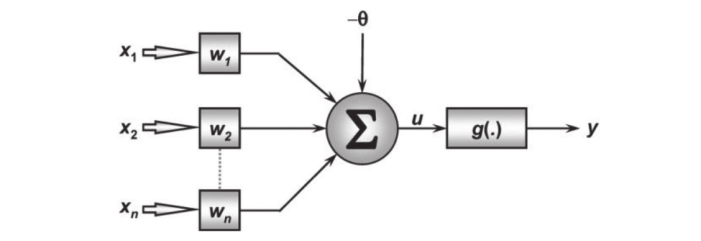
\includegraphics[keepaspectratio=true,scale=0.5]{figuras/neuronio_artificial.png}
	\caption{Neurônio Artificial \cite{silva}}
\end{figure}

A representação matemática do relacionamento entre os nós, pesos e vieses é descrita na Equação \ref{eq_rna}. A soma dos pesos de entrada para uma camada passa pela função de ativação não linear para outro nó da próxima camada. O que pode ser interpretado como um vetor, onde {$x_i$} são inputs e {$w_i$} são os pesos, {$f$} é a função de ativação e, por fim, {$Z$} é a saida.

\begin{equation}
\label{eq_rna}
	Z = f(x.w+b) = f(\sum_{i=1}^n (x_i^T w_i + b))
\end{equation}

Calculando os pesos e vieses, o processo de treinamento é completado quando: A inicialização dos pesos e vieses de todos os nós deve ser feita de forma aleatória, realizando uma passagem para frente dos atuais pesos e vieses e calculando a saída de cada nó, e modificando os pesos e vieses consequentemente pelo gradiente descendente com passagem para trás, processo conhecido pelo termo em ingês \emph{backpropagation algorithm} \cite{rna3}


\subsection{Redes Neurais Convolucionais}

Redes Neurais Convolucionais, mais conhecidas como CNN's, originda do termo em inglês (\emph{Convolutional Neural Network}) é muito inspirada no processo biológico de processamentos de dados visuais. Uma CNN é capaz de aplicar filtros de dados visuais, mantendo semelhança de vizinhança entre os pixels da imagem ao longo do processamento da rede, o que permitiu o método ganhar bastante espaço no ambito de visão computacional com aplicações na classificação, detecção e reconhecimento em imagens e vídeos. \cite{rnc} 

Uma CNN é composta pelas seguintes camadas: camada convolucional, camada de agrupamento e camada totalmente conectada. Onde a camada convolucional utiliza filtros sobre a imagem  afim de obter uma série de mapas de características para cada filtro. As camadas de agrupamento são responsáveis por reduzir a amostra para os mapas de características e, ao fim, a tarefa de classificação das imagens é realizada pela camada totalmente conectada. \cite{rnc2} Podemos ver um exemplo de uma CNN e suas diversas camadas na Figura \ref{fig_rnc}

\begin{figure}[!h]
	\centering
	\label{fig_rnc}
		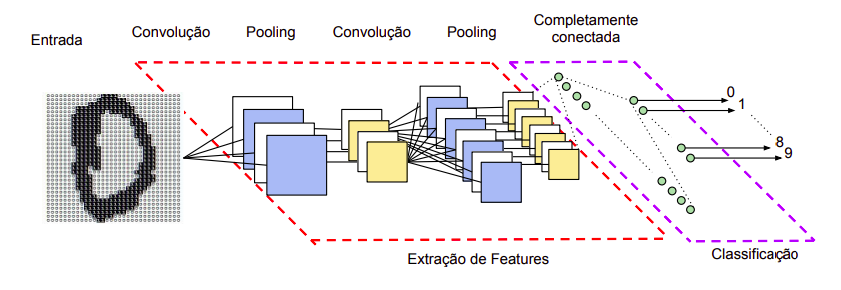
\includegraphics[keepaspectratio=true,scale=0.5]{figuras/exemplo_convolucao.png}
	\caption{Exemplo de uma rede neural convolucional \cite{rnc}}
\end{figure}


Além da sua vasta aplicação no ambito da visão computacional, as variações de arquiteturas de Redes Neurais Convolucionais veem obtendo bons resultados em outras áreas de aplicação.\cite{rnc4} utilizaram CNNs Dinâmicas para uma série de tarefas de Processamento Natural de Linguagens como análise de sentimentos e classifiação de tipos de pergunta.\cite{rnc5} utilizaram o método para classificação binária de frases como positivo ou negativo.\cite{rnc3}

\subsection{Redes Neurais Recorrentes}

As redes neurais recorrentes, do inglês (\emph{recurrent neural networks} - RNN) são um caso especial onde existe realimentação de entradas\cite{rnn2} conforme ilustrado na Figura \ref{fig_rnn}. A realimentação faz com que as redes neurais apresentem um comportamento dinâmico temporal. Por apresentarem capacidade de memória, ou seja, habilidade de armazenar informação de dados anteriores, são muit utilizadas em questões relacionadas a séries temporais. Uma rede neural recorrente pode responder a mesma entrada com diferentes saídas em diferentes momentos, dependendo da entrada apresentada anteriormente \cite{rnn}.

\begin{figure}[!h]
	\centering
	\label{fig_rnn}
		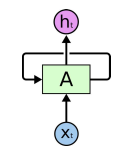
\includegraphics[keepaspectratio=true,scale=0.4]{figuras/exempo_rede_neural_recorrente.png}
	\caption{Rede neural Recorrente \cite{rnn3}}
\end{figure}

A figura \ref{fig_rnn} mostra uma exemplificação de uma RNN em um instante de tempo {$t$} e uma entrada {$x_i$} produzindo uma saída {$h_t$}. Onde a camada {$A$} é recorrente. Outro modo de visualizar as redes neurais é expandindo suas recorrências, como demonstrado na figura \ref{fig_rnn2}. Desta forma é possível visualizar o fluxo de dados de uma RNN, sendo essa uma expansão da rede mostrada na \ref{fig_rnn};.

\begin{figure}[!h]
	\centering
	\label{fig_rnn2}
		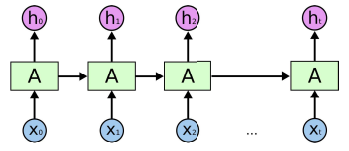
\includegraphics[keepaspectratio=true,scale=0.5]{figuras/Exemplo_Rnn_expandido.png}
	\caption{Rede Neural Recorrente Expandida \cite{rnn3}}
\end{figure}

\subsubsection{Long Short-Term Memory}

As redes \emph{Long short-term Memory} (LSTM) são um tipo especial de RNN que permite solucionar problemas de explosão e desvanecimento de gradientes em RNNs, capazes de aprender informações de longo prazo, sendo primeiramente introduzidas por Hochreiter e Schmidhuber \cite{lstm1}. LSTMs são bastante utilizadas quando o volume de dados é muito grande e as informações anteriores tornam-se de longo prazo, geralmente apresetando resultados melhores em comparaçao as RNNs.

A principal diferença entre as RNNs e uma LSTM é que em cada neurônio da LSTM há uma célula de memória. Onde cada neurônio possui três \emph{gates}, sendo eles: \emph{gate} de entrada, \emph{gate} de equecimento e \emph{gate} de saída \cite{rna3}, conforme ilustrado na Figura \ref{fig_lstm1}, onde é utilizado a função sigmoide {$\sigma$} nos \emph{gates} de regulagem e a função \emph{tanh} nos \emph{gates} análogos a função de recompensa.

\begin{figure}[!h]
	\centering
	\label{fig_lstm1}
		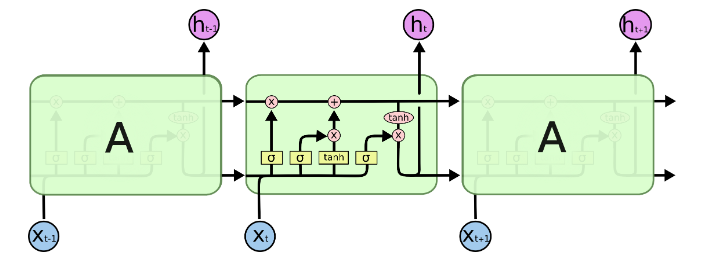
\includegraphics[keepaspectratio=true,scale=0.5]{figuras/lstm.png}
	\caption{Exemplo Long Short-Term Memory \cite{rnn3}}
\end{figure}

A primeira operação realizada dentro da LSTM é a remoção das memórias, executada pelo \emph{gate} de esquecimento representado na equacao \ref{eq_lstm1}

\begin{equation}
\label{eq_lstm1}
	f_t = \sigma (W_f [h_{t-1}, X_t]+b_f)
\end{equation}

Para definir as informações que será armazenada no estado da célula, é preciso realizar dois processos. Primeiramente é camada chamada de \emph{gate} de entrada decide qual valor será atualizado, logo após, uma camada tangencial cria um vetor {$\widetilde{C_t}$} e em seguida é combinado o \emph{gate} de entrada com o vetor para realizar a atualização do estado, conforme mostrado na Equação \ref{eq_lstm2} e na Equação \ref{eq_lstm3}. 

\begin{equation}
\label{eq_lstm2}
	i_t = \sigma (W_i [h_{t-1}, X_t]+b_i)
\end{equation}

\begin{equation}
\label{eq_lstm3}
    \widetilde{C_t}=  tanh(W_C [h_{t-1}, X_t]+b_C)
\end{equation}

Por fim, é deletado a informação antiga e adicionado as novas informações definidas nas etapas anteriores. Atualizando o instante no tempo {$t$}, conforme descrito na Equação \ref{eq_lstm4}.

\begin{equation}
\label{eq_lstm4}
    C_t =  f_t * C_{t-1} + i_t * \widetilde{C_t}
\end{equation}

O \emph{gate} de saída será definido pela célula de estado filtrada. Onde é aplicado uma função sigmoide na entrada {$h_{t-1}$} e {$X_t$}, como representado na Equação \ref{eq_lstm5}.

\begin{equation}
\label{eq_lstm5}
    o_t = \sigma(W_o [h_{t-1}, X_t] + b_o)
\end{equation}

Finalmente, o \emph{gate} de saída é multiplicada por uma camada tangencial do estado da célula para termos a saída desejada no instante de tempo {$t$}, conforme a Equação \ref{eq_lstm6}

\begin{equation}
\label{eq_lstm6}
    h_t = o_t * tanh(C_t)
\end{equation}

\section{Métricas de Avaliação}
\label{mav}

Algoritmos de inteligência artificial e \emph{Deep Learning} são averiguados em todas as fases do processo, desde a validação à testagem. Diversas linguagens possuem \emph{frameworks} que auxiliam nos cálculos de diversos parâmetros que podem ser úteis na avaliação do algorítmo. É usual interpretaçoes simplistas que exibem exclusivamente situações de classificações binárias, e conforme o aumento da complexidade, são comuns equívocos na classificação.\cite{ma3}

Neste contexto, este tópico visa exemplificar e definir os principais parâmetros de avaliação utilizados nos classificadores de \emph{Machine Learning} e \emph{Deep Learning}, sendo eles: Erro Percentual Absoluto médio, Erro Médio Absoluto, Erro Relativo da Raiz Média Quadrada, Erro Quadrático Médio, Acurácia, Precisão, Recall e F1-Scores.

\subsection{Erro Percentual Absoluto Médio}

O Erro Percentual Absoluto Médio, mais conhecidamente pelo seu termo em inglês \emph{Mean Absolute Percentage Error} (MAPE) é uma medida de erro relativo, que usa valores absolutos para impossibilitar que os erros positivos e negativos se anulem e assim, usa os erros relativos para permitir que haja uma comparação entre a precisão da previsão nos métodos de séries temporais \cite{oracle}, sendo sempre apresentada em forma de porcentagem, conforme a Equação \ref{mape}.

\begin{equation}
\label{mape}
    MAPE = \frac{1}{n} \sum_{t=1}^n (\mid \frac{A_t - F_t}{A_t} \mid)* 100)
\end{equation}

Onde, {$A_t$} é o valor atual e {$F_t$} é o valor previsto. Pela fórmula, O valor absoluto é a diferença entre o valor real e previsto dividido pelo valor real. Por fim, o erro é multiplicado por 100 para ficar na forma percentual.

\subsection{Erro Médio Absoluto}

O Erro Médio Absoluto ou \emph{Mean absolute Error} (MAE) é uma métrica de avaliação bastante usada avaliação de modelos. O MAE é medido pela média entre dois valores, sendo eles {$A_t$} e {$F_t$}, representando respectivamente o valor real e o valor da predição, como demonstrado na equação \ref{mae}.

\begin{equation}
\label{mae}
    MAE = \frac{1}{n} \sum_{t=1}^n \mid A_t - F_t \mid
\end{equation}

Onde {$n$} representa o número de amostras.

\subsection{Erro Relativo da Raiz Média Quadrada}

O Erro da Raiz Média Quadrada (RMSE) do inglês \emph{Root Mean Square Error} representa o desvio padrão dos erros de previsão no modelo de regressão trabalhado. Os Erros de previsão, mostram a distância entre os valores reais e os valores previstos na modelagem. A métrica é utilizada para indicar como está a concentração dos dados perto do melhor modelo treinado. O Erro Relativo da Raiz Quadrada, ou RRMSE do inglês \emph{Relative Root Mean Square Error} seria uma variação do RMSE, onde o erro quadrático total é normalizado e dividido pelo erro quadrático total previsto\cite{rna3}, como descrito pela Equação \ref{rrmse}

\begin{equation}
\label{rrmse}
    RRMSE = \sqrt{\frac{1}{n} \sum_{t=1}^n  (\frac{A_t - F_t}{A_t})^2}
\end{equation}

Onde {$A_t$} representa o valor real, {$F_t$} o valor previsto e {$n$} o tamanho da amostra

\subsection{Erro Quadrático Médio}

O Erro Quadrático Médio (\emph{Mean Squared Error}, MSE) mensura a qualidade das predições e o valor não negativo, onde quanto mais perto de 0 for a métrica, melhor será a qualidade das predições do modelo. O MSE demonstra o quão amplamente espalhadas as previsões são de uma amostra para outra, e o quão próximo o valor médio previsto está da observação \cite{ma2}. Como pode ser exemplificado pela Equação \ref{mse}

\begin{equation}
\label{mse}
    MSE = \frac{1}{n} \sum_{t=1}^n  (A_t - F_t)^2
\end{equation}

Onde {$A_t$} representa o valor real, {$F_t$} o valor previsto e {$n$} o tamanho da amostra

\subsection{Acurácia}

A acurácia é amplamente utilizada como parâmetro central na avaliação de classificadores na inteligência artificial, principalmente pela sua simplicidade de compreensão.\cite{ma3}

A Acurácia mede o percentual de casos verdadeiros em relação a todos os resultados, podendo ser calculada então como a razão entre o número total de observações certas do modelo e o total de observações previstas, conforme a Equação \ref{acuracia}.

\begin{equation}
\label{acuracia}
    Acuracia = \frac{V_p + V_n}{V_p + F_n + F_p + V_n}
\end{equation}

Onde, {$V_p$} é o número de amostras com classificação correta positivas, {$V_n$} o número de amostras com classificação correta negativas, {$F_p$} número de amostras que o modelo previu como verdadeiro, quando o valor real é negativo e por fim, {$F_n$} que é o número de amostras que o modelo previu negativo quando o valor real da classe era positivo.

\subsection{Precisão}

A precisão mede a relação entre as amostras previstas como verdadeiras e positivas e o total previsto. Conforme a Equação \ref{precisao}

\begin{equation}
\label{precisao}
    precisão = \frac{V_p}{T_p + F_p}
\end{equation}

Onde, {$V_p$} são os verdadeiros positivos e {$F_p$} são os falso positivos. Podemos perceber pela relação que ao elevar a quantidade de falso positivos, a precisão do algorítmo cai. Geralmente a precisão é avaliada quando o peso dos falso positivos é relativo para o problema que se quer solucionar.

\subsection{Retorno}

O retorno, ou como é mais conhecido do inglês \emph{Recall} trata da porcentagem de todos os verdadeiro positivos previstos corretamente. Conforme a Equação \ref{recall}

\begin{equation}
\label{recall}
    retorno = \frac{V_p}{T_p + F_n}
\end{equation}

Onde, {$V_p$} representam os verdadeiros positivos e {$F_n$} representam os falso negativos. Pela relação demonstrada, o peso dos {$F_n$} é maior em relação ao {$F_p$} no modelo avaliado. Mede a taxa de verdadeiro positivos que o modelo prediz, possibilitando analisar a capacidade do classificador na identificação dos {$F_n$} \cite{ma3}.
 
\subsection{F1-Scores}

O F1 score funciona como a média harmônica entre a precisão e o retorno, funciona como uma métrica unificada de ambos, atribuindo um peso maior aos valores menores, em relação a uma média aritmética simples. Como demonstrado na Equação \ref{f1}  

\begin{equation}
\label{f1}
    F1 = \frac{2 * precisão * retorno}{precisão + retorno}
\end{equation}

\section{Trabalhos Correlatos}
\label{tc}

A predição do mercado de ações em qualquer ambito tem sido um tópico bastante explorado e pesquisado a muito tempo, embora a maior parte das pesquisas do uso de técnicas de Machine Learning e principalmente Deep learning no mercado financeiro é relativamente recente. 

O estudo de \cite{rna3} utiliza dados históricos de 10 anos dos índices nos grupos de finanças, petróleo, minerais não metálicos e metáis básicos da Bolsa de Valores de Teerã para prever dados de 1, 2, 5, 10, 15, 20 e 30 dias a frente, realizando uma comparação entre diversos tipos de algorítmos de \emph{Machine} e \emph{Deep Learning}, como: \emph{decision tree, bagging, random forest, adaptive boosting (Adaboost), gradient boosting, and eXtreme gradient boosting (XGBoost), artificial neural networks (ANN), recurrent neural network (RNN)} e \emph{long short-term memory (LSTM)}. Para mensuração e avaliação dos resultados, foram utilizadas algumas das medidas de erro descritas no capítulo \ref{mav} sendo as abordadas pelo estudo: MAPE, MAE, RRMSE, MSE. O estudo realizado, chegou ao resultado de que pelos algorítmos e dados utilizados, LSTM apresenta resultados mais acertivos e uma alta capacidade de ajuste do modelo. 

O artigo \cite{tc6} avalia a série temporal diária do valor de fechamento de alguns dos principais índices mundiais em termos de volumetria de negociação como o {S\&P500}, Down Jones, Nasdaq e Shanghai Stock Exchange entre as datas de 4 de Janeiro de 2010 a 31 de Dezembro de 2018, observando 2272 dias de transações. O estudo traz uma comparação entre o modelo desenvolvido, chamado de \emph{RC Model} e os métodos mais utilizados de RNN e LSTM, onde o modelo proposto apresenta resultados bastante próximos e em alguns aspectos até mesmo melhor que das arquiteturas convencionais de LSTM e RNN.

O trabalho de \cite{tc2} apresenta um estudo utilizando uma abordagem híbrida, integrando uma rede LSTM com um algorítmo genético (GA) na predição do índice de da Bolsa de Valores da Korea (KOSPI), conforme o fluxograma da Figura \ref{fluxo_GA-LSTM}.

\begin{figure}[!h]
	\centering
	\label{fluxo_GA-LSTM}
		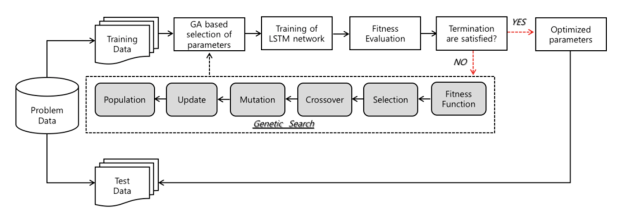
\includegraphics[keepaspectratio=true,scale=0.6]{figuras/fluxograma_ga_lstm.png}
	\caption{ Fluxograma do modelo GA-LSTM \cite{tc2}}
\end{figure}

O estudo contou com dados de Janeiro de 2000 a Dezembro de 2016, contando com 4203 dias de transações, analisando dados de: valor de venda diário, menor preço, maior preço, preço de abertura, preço de fechamento e volume transacionado. Foi analisado as métricas de MSE, MAE e MAPE, onde o modelo teve resultados consideravelmente melhores em relação ao \emph{Benchmark} comparado.


O artigo elaborado por \cite{tc3} realizou um estudo comparando diversas arquiteturas de LSTM e GRU. O artigo analisa dados do dia 03 de Março de 2010 ao dia 17 de Setembro de 2019, totalizando 2403 dados de treinamento das ações: AMZN e GOOGL, BLL, QCOM. Para avaliar os modelos, foram avaliados as métricas de erro: MAPE, RMSPE e RMSDE, onde foi analisado que ambos modelos tiveram bons resultados em todas as arquiteturas analisadas, mantendo acurácias na faixa de 92,74\% a 98,47\% para o MAPE percentual, 90,44\% a 97,96\% para o RMSPE e 66,64\% a 90,73\% para RMSDE.

Os principais resultados dos estudos citados anteriormente e outros relevantes para composição do trabalho podem ser visualizados nas tabelas \ref{literatura_deep_learning} e \ref{literatura_machine_learning}, onde é apresentado os modelos analisados, as métricas de avaliação, os resultados obtidos e as referências de quem realizou cada pesquisa. 


\begin{table}[H]

\begin{tabular}{@{}llll@{}}
\toprule
\textbf{Modelo} & \textbf{Métrica}                                                 & \textbf{Resultado}                                                     & \textbf{Literatura}                                \\ \midrule
RNN             & \begin{tabular}[c]{@{}l@{}}MAPE\\ MAE\\ RRMSE\\ MSE\end{tabular} & 
\begin{tabular}[c]{@{}l@{}}1,85\\ 17,20\\ 0,0281\\ 635,85\end{tabular} & \cite{rna3}                                         \\ \\ 
LSTM            & \begin{tabular}[c]{@{}l@{}}MAPE\\ MAE\\ RRMSE\\ MSE\end{tabular} & \begin{tabular}[c]{@{}l@{}}0,6\\ 6,7\\ 0,0093\\ 148,77\end{tabular}    &                                                    \\ \midrule
LTSM            & \begin{tabular}[c]{@{}l@{}}MAPE\\ MAE\end{tabular}               & \begin{tabular}[c]{@{}l@{}}0,66\\ 20,78\end{tabular}                   & \cite{tc1}          \\ \midrule
GA-LSTM            & \begin{tabular}[c]{@{}l@{}}MAPE\\ MAE\end{tabular}               & \begin{tabular}[c]{@{}l@{}}0,91\\ 10,21\end{tabular}                   & \cite{tc2}                        \\ \midrule
LSTM            & \begin{tabular}[c]{@{}l@{}}MAPE\\ RRMSE\end{tabular}             & \begin{tabular}[c]{@{}l@{}}0,96\\ 0,95\end{tabular}                    & \cite{tc3}                        \\ 
GRU             & \begin{tabular}[c]{@{}l@{}}MAPE\\ RRMSE\end{tabular}             & \begin{tabular}[c]{@{}l@{}}0,97\\ 0,96\end{tabular}                    &                                                    \\ \midrule
LSTM            & \begin{tabular}[c]{@{}l@{}}MAE\\ RMSE\end{tabular}               & \begin{tabular}[c]{@{}l@{}}38,35\\ 47,96\end{tabular}                  & \cite{tc5} \\ \\ 
GRU             & \begin{tabular}[c]{@{}l@{}}MAE\\ RMSE\end{tabular}               & \begin{tabular}[c]{@{}l@{}}31,82\\ 43,16\end{tabular}                  &                                                    \\ \\ 
RNN             & \begin{tabular}[c]{@{}l@{}}MAE\\ RMSE\end{tabular}               & \begin{tabular}[c]{@{}l@{}}15,37\\ 23,44\end{tabular}                  &                                                    \\ \midrule
LSTM            & \begin{tabular}[c]{@{}l@{}}RMSE\\ MAE\end{tabular}               & \begin{tabular}[c]{@{}l@{}}23,89\\ 15,66\end{tabular}                  & \cite{tc6}                           \\ \\
RC Model            & \begin{tabular}[c]{@{}l@{}}RMSE\\ MAE\end{tabular}               & \begin{tabular}[c]{@{}l@{}}23,25\\ 15,80\end{tabular}                  &                           \\ \\ 
RNN            & \begin{tabular}[c]{@{}l@{}}RMSE\\ MAE\end{tabular}               & \begin{tabular}[c]{@{}l@{}}23,44\\ 15,37\end{tabular}                  &                           \\ \midrule

CNN             & \begin{tabular}[c]{@{}l@{}}MAPE\\ RRMSE\end{tabular}             & \begin{tabular}[c]{@{}l@{}}0,52\\ 0,81\end{tabular}                     &  \cite{tc8}                                                      \\
\bottomrule
\end{tabular}
\caption{Resultados relevantes de métodos de Deep Learning}
\label{literatura_deep_learning}
\end{table}

\begin{table}[H]
\centering

\begin{tabular}{@{}llll@{}}
\hline
\textbf{Modelo} & \textbf{Métrica} & \textbf{Resultado}  & \textbf{Literatura}                
\\ \midrule

Decision Tree  & \begin{tabular}[c]{@{}l@{}}MAPE\\ MAE\\ RRMSE\\
MSE\end{tabular} & \begin{tabular}[c]{@{}l@{}}2,07\\35,82\\0,0396\\7984,3\end{tabular}  & \cite{rna3}    \\ \\

Random Forest  & \begin{tabular}[c]{@{}l@{}}MAPE\\ MAE\\ RRMSE\\
MSE\end{tabular} & \begin{tabular}[c]{@{}l@{}}1,91\\ 31,96\\ 0,0288\\ 3962,97\end{tabular}   \\ \\

Adaboost & \begin{tabular}[c]{@{}l@{}}MAPE\\ MAE\\ RRMSE\\ MSE\end{tabular}  & \begin{tabular}[c]{@{}l@{}}1,59\\ 26,27\\ 0,0248\\ 2867,63\end{tabular}   \\ \midrule

Decision Tree  & \begin{tabular}[c]{@{}l@{}}APE\\ RRMSE\end{tabular}               & \begin{tabular}[c]{@{}l@{}}0,59\\ 0,87\end{tabular}                   & \cite{tc8}
\\
\bottomrule
\end{tabular}
\caption{Resultados relevantes de métodos de Machine Learning}
\label{literatura_machine_learning}
\end{table}


\section{Considerações Finais}
\label{cf}

O capítulo apresentou definições e contextualização sobre os principais tópicos abordados nesse trabalho. Iniciamos com a contextualização do mercado de ações e como ela funciona no Brasil, descrevemos a motivação para predição do índice do Bovespa e sua composiçaõ atual, exemplificamos os principais métodos de Deep Learning para análise predição de séries temporais, as métricas de avaliação de modelos de inteligência artificial e por fim, descrevemos os principais trabalhos correlatos com o objetivo deste trabalho.

Com a análise dos estudos, vimos como as técnicas foram aplicadas para a problemática da predição do valor das ações e os resultados obtidos por cada estudo. Entendemos as  \emph{features} utilizadas e como foi mensurado os resultados de cada modelo, desta forma, é possível utilizar as melhores ideias dos estudos analisados durante a pesquisa para composição deste trabalho.
